Obviously, training and evaluation of a knowledge graph completion model require a knowledge graph. In case of the Power model, there is also the need for textual entity descriptions. The graphs chosen for this work are the popular FB15K-237~\cite{Toutanova2015ObservedVL} subset of the  Freebase~\cite{Bollacker2008FreebaseAC} graph and the CoDEx~\cite{Safavi2020CoDExAC} graph, a knowledge graph constructed with the aim of providing a further improved benchmark for knowledge graph completion. The graphs' fact splits into training, validation and test subsets, together with matching texts, are provided by Felix Hamann as part of his work on inductive reasoning with Text (IRT), an approach to create open-world evaluation benchmarks from given knowledge graphs~\cite{}. The following \autoref{subsec:5_experiments/1_data_sources/1_knowledge_graphs} and \autoref{subsec:5_experiments/1_data_sources/2_text_sets} give an impression of the size of the knowledge graphs, the shape of the fact splits and the kind of texts in the text sets.

\subsection{Knowledge Graphs}
\label{subsec:5_experiments/1_data_sources/1_knowledge_graphs}
One of the most popular knowledge graphs is Freebase~\cite{Bollacker2008FreebaseAC}. Although it is not maintained anymore since it was integrated into Wikidata in 2015~\cite{Tanon2016FromFT}, the benchmark datasets derived from it are still widely used. One of those benchmark datasets is the \emph{FB15k} dataset introduced by Bordes et al. in 2013~\cite{Bordes2013TranslatingEF}, which covers roughly \num{15000} Freebase entities. On its basis, Toutanova and Chen introduced the FB15k-237 subset in 2015~\cite{Toutanova2015ObservedVL}, whose purpose was to create a more meaningful benchmark by eliminating trivially predictable facts. For example, if FB15k-237 covers a relation like $(x, contains, y)$, it does not include its inverse relation $(y, part~of, x)$, because good performance resulting from such trivial, mutual predictions detracts from more interesting cases. In 2020, Safavi and Koutra published another dataset called CoDEx~\cite{Safavi2020CoDExAC}, which is derived from FB15k-237 and two other datasets, covers more diverse content and in turn poses a greater challenge than FB15k and FB15k-237. From the three provided variants of the CoDEx dataset -- CoDEx-S, CoDEx-M, and CoDEx-L -- the IRT approach by Hamann, on which this work is based, focuses on the CoDEx-M dataset. \autoref{tab:5_experiments/1_data_sources/1_knowledge_graphs/benchmark_datasets} gives an overview of the scales of FB15k, FB15k-237 and CoDEx-M. CoDEx-M actually contains additional, negative facts that are excluded here as this work focuses on the common open-world scenario.

\begin{table}[h]
    \centering
    \begin{tabular}{| l | r | r | r | r | r |}
    \hline

    \multicolumn{1}{|c|}{\textbf{Dataset}} &
    \multicolumn{1}{|c|}{\textbf{#Entities}} &
    \multicolumn{1}{|c|}{\textbf{#Relations}} &
    \multicolumn{3}{|c|}{\textbf{#Facts}} \\

    \multicolumn{1}{|c|}{} &
    \multicolumn{1}{|c|}{} &
    \multicolumn{1}{|c|}{} &
    \multicolumn{1}{|c|}{\textbf{Train}} &
    \multicolumn{1}{|c|}{\textbf{Valid}} &
    \multicolumn{1}{|c|}{\textbf{Test}} \\

    \hline \hline

    FB15k     & \num{14951} & \num{1345} & \num{483142} & \num{50000} & \num{59071} \\
    FB15k-237 & \num{14541} & \num{237}  & \num{272115} & \num{17535} & \num{20466} \\
    CoDEx-M   & \num{17050} & \num{51}   & \num{185584} & \num{10310} & \num{10311} \\

    \hline
\end{tabular}

    \caption{Comparison of popular KGC benchmark datasets}
    \label{tab:5_experiments/1_data_sources/1_knowledge_graphs/benchmark_datasets}
\end{table}

As for the above KGC benchmark datasets, a graph's fact set is usually further split into training, validation, and test subsets. Thereby, the splits are created so that there are training, validation, and test facts for possibly every entity. In contrast to that common approach, in his work on zero-shot learning, Hamann creates new \emph{IRT splits} from FB15k-237 and CoDEx-M that distinguish between so-called \emph{closed-world (CW) entities}, that are seen during training, and \emph{open-world (OW) entities}, which are not seen during training, to optimize prediction for unknown entities.

\begin{figure}
    \centering
    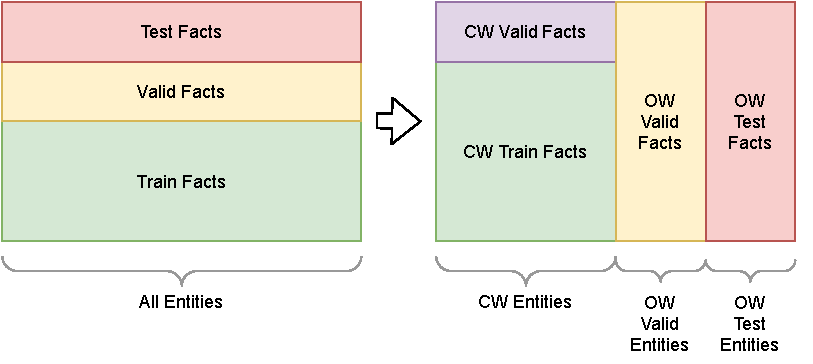
\includegraphics[width=\textwidth]{5_experiments/1_data_sources/1_knowledge_graphs/irt_split}
    \caption{Difference between a conventional and an IRT fact split. The IRT fact split focuses on open-world entities that must stay unseen during training. ``CW'' = ``closed-world'', ``OW'' = ``open-world''.}
    \label{fig:5_experiments/1_data_sources/1_knowledge_graphs/irt_split}
\end{figure}

\autoref{fig:5_experiments/1_data_sources/1_knowledge_graphs/irt_split} illustrates the different shape of an IRT fact split compared to a conventional one: The closed-world entities' facts are split into closed-world training and closed-world validation facts to enable closed-world prediction. Meanwhile, the open-world entities' facts are completely reserved for validation and training, respectively. Closed-world training and closed-world validation facts only refer to closed-world entities. On the other hand, one of an open-world validation fact's head or tail may also be a closed-world entity, and one of an open-world test fact's head or tail may be a closed-world entity or an open-world validation entity. \autoref{tab:5_experiments/1_data_sources/1_knowledge_graphs/irt_splits} gives an overview of the scales of the IRT splits' entity and fact subsets.

\begin{table}[h]
    \centering
    \begin{tabular}{ l c r r r c r r c r r }
    \toprule
    
    \multicolumn{1}{l}{\textbf{Graph}} & \phantom &
    \multicolumn{1}{c}{\textbf{\thead{CW \\ Train \\ Ents}}} &
    \multicolumn{1}{c}{\textbf{\thead{CW \\ Train \\ Facts}}} &
    \multicolumn{1}{c}{\textbf{\thead{CW \\ Valid \\ Facts}}} & \phantom &
    \multicolumn{1}{c}{\textbf{\thead{OW \\ Valid \\ Ents}}} &
    \multicolumn{1}{c}{\textbf{\thead{OW \\ Valid \\ Facts}}} & \phantom &
    \multicolumn{1}{c}{\textbf{\thead{OW \\ Test \\ Ents}}} &
    \multicolumn{1}{c}{\textbf{\thead{OW \\ Test \\ Facts}}} \\

    \midrule

    FB15k-237 && \num{12057} & \num{214412} & \num{23778} && \num{1545} & \num{46503} && \num{816}  & \num{25423} \\
    CoDEx-M   && \num{11399} & \num{123650} & \num{13738} && \num{2918} & \num{41240} && \num{1896} & \num{27577} \\

    \bottomrule
\end{tabular}

    \caption{Scale of the IRT splits of the FB15k-237 and CoDEx-M datasets}
    \label{tab:5_experiments/1_data_sources/1_knowledge_graphs/irt_splits}
\end{table}


\subsection{Text Sets}
\label{subsec:5_experiments/1_data_sources/2_text_sets}
In addition to the open-world fact splits of FB15k-237 and CoDEx-M, Hamann provides multiple text sets for each split's entities. Thereby, the text sets' contents vary in quality and quantity, ranging from text sets that offer single, very specific entity descriptions to text sets that provide multiple low-quality contexts not necessarily describing the entity directly. Some of the text sets contain plain text, some mark the entity's mentions within the text via special tokens, and some mask the entity mention. Together with the choice between FB15k-237 and CoDEx-M, this allows for graph-text combinations suiting different real-world scenarios.

Table~\ref{tab:5_experiments/1_data_sources/2_text_sets/text_sets_table} lists some example sentences from selected text sets and shortly describes the naming schema behind the text sets' names that will be used throughout this chapter, while Table~\ref{tab:a_appendix/text_sets_all} in Appendix~\ref{ch:a_appendix} lists all text sets. For example, the text set named "cde-irt-5-marked" indictates that it contains up to five marked sentences for each entity in the CoDEx-M graph. Thereby, the four dash-separated name parts denote (1) the graph for whose entities texts are provided, (2) the texts' origin, (3) the maximum number of sentences per entity and (4) whether the sentences are marked masked. There are three types of sentences that are distinguished by their source:

\begin{itemize}
    \item The \emph{CDE sentences} were provided by the authors of the CoDEx paper~\cite{}. They are the entities' first sentence from their respective Wikipedia page and thus very specific.
    \item The \emph{IRT sentences} have been introduced in Hamann's IRT paper~\cite{}. They are randomly sampled entity contexts from the English Wikipedia that mention the entity in a more or less meaningful way anywhere in the sentence.
    \item The \emph{OWE sentences} are very compact entity descriptions, often consisting of only a few words. They were created by Villmov et al. during the work on their OWE model for open-world KGC~\cite{Shah2019AnOE}.
\end{itemize}

\begin{table}
    \centering
    \begin{tabularx}{\textwidth}{ l >{\hsize=.42\hsize}X >{\hsize=.58\hsize}X }
    \toprule
    
    \multicolumn{1}{l}{\textbf{Text Set}} &
    \multicolumn{1}{l}{\textbf{Description}} &
    \multicolumn{1}{l}{\textbf{Example}} \\
    
    \midrule
    
    cde-cde-1-clean & One CDE sentence per CDE entity &
    A Few Good Men is a 1992 American legal drama film directed by Rob Reiner and starring \dots \\ 
    
    \midrule
    
    cde-irt-5-marked & Up to five marked IRT sentences per CDE entity &
    \dots for Best Film Editing for the feature film, [START] A Few Good Men [END] (1992). \\ 

    \midrule
    
    fb-irt-30-masked & Up to 30 masked IRT sentences per FB entity &
    The [MASK] has qualified one male and one female athlete in the artistic gymnastics competition. \\ 

    \midrule
    
    fb-owe-1-clean & One OWE sentence per FB entity &
    Country in the caribbean. \\

    \bottomrule
\end{tabularx}

    \caption{Example sentences from some of the text sets. The text set name a-b-c-d reveals (a) the graph ("fb" = FB15k-237, "cde" = CoDEx-M), (b) the text origin ("cde", "irt", "owe"), (c) the maximum number of sentences per entity and (d) whether entity mentions are marked or masked.}
    \label{tab:5_experiments/1_data_sources/2_text_sets/text_sets_table}
\end{table}

